%
% This work is licensed under a Creative Commons Attribution-ShareAlike 4.0 International License.
% http://creativecommons.org/licenses/by-sa/4.0/
%

% DO NOT COMPILE THIS FILE DIRECTLY!
% This is included by the other .tex files.


\begin{frame}
    \includegraphics[scale=0.3]{images/logo-circl-Forensics.png}
    \begin{itemize}
        \item[]
        \item[]
        \item[] 4. Basic Malware Analysis
    \end{itemize}
\end{frame}


\begin{frame}[fragile]
  \frametitle{4.1 Introduction}
    \begin{itemize}
	    \item[] Take care: Self-Infection:
    	    \begin{itemize}
	    	\item Keep away from production
		\item Isolated machines (VMs)
		\item Network considerations
		\item[]
    	    \end{itemize}
	    \item[] Exchange of malware via email:
    	    \begin{itemize}
	    	\item Password protected archive
		\item Password: \texttt{infected}
		\item[]
    	    \end{itemize}
	    \item[] 5 Phases of analysis
            \begin{enumerate}
            	\item OSINT - Open Source Intelligence
		\item Automatic Analysis (Sandbox)
            	\item Static Analysis
		\item Dynamic Analysis (Behavioral Analysis)
            	\item Reverse Engineering
		\item[]
            \end{enumerate}
    \end{itemize}
\end{frame}


\begin{frame}[fragile]
  \frametitle{4.2 OSINT - IoCs}
    \begin{itemize}
	    \item Is the file \texttt{Form.exe} malicious?
            \item What it is doing?
    \end{itemize}
  \begin{lstlisting}[basicstyle=\tiny]
    ls -l Form.exe				                    189952 Form.exe
   md5sum Form.exe		                   a8371cb187d99711691ccbecf8f35657
  sha1sum Form.exe                         8dec32121d2f9f876c2b157451968796608d3dd5
sha256sum Form.exe 784560f38065089f1c61869f7ebdc58b0115d500e5113e6c09d1b4d885ccb340
  \end{lstlisting}
  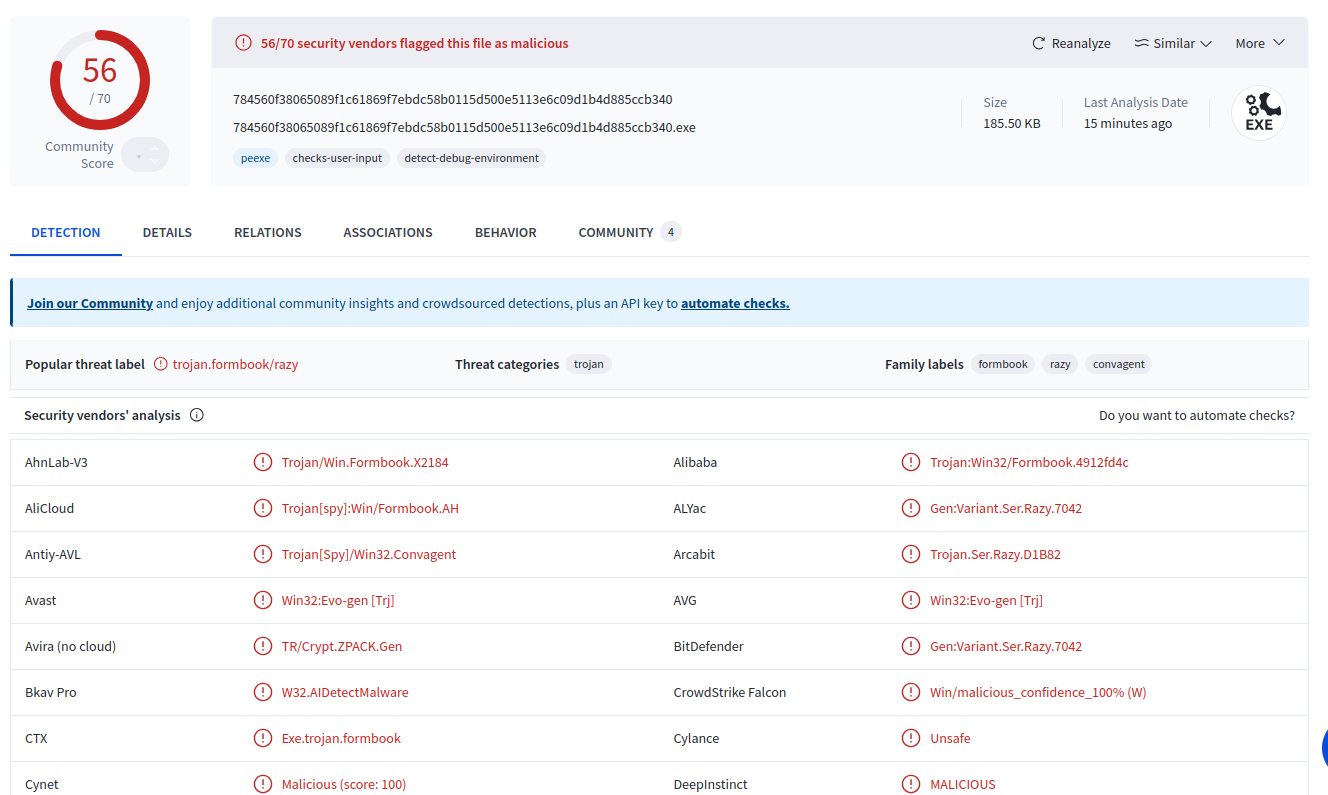
\includegraphics[scale=0.17]{images/VT_1.png}
\end{frame}


\begin{frame}[fragile]
  \frametitle{4.2 OSINT - Malpedia}
  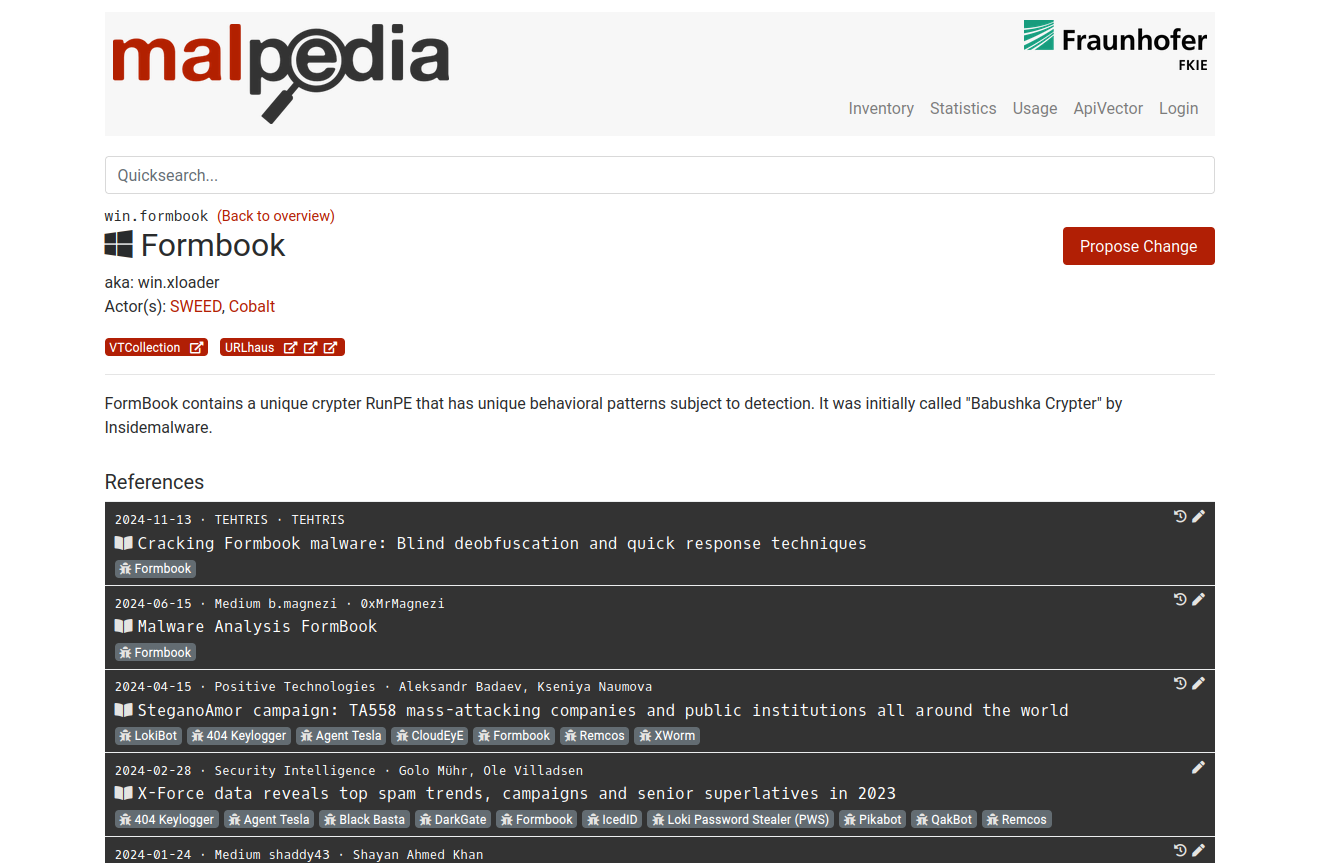
\includegraphics[scale=0.24]{images/malpedia.png}
\end{frame}


\begin{frame}[fragile]
  \frametitle{4.2 OSINT - VirusTotal Details}
  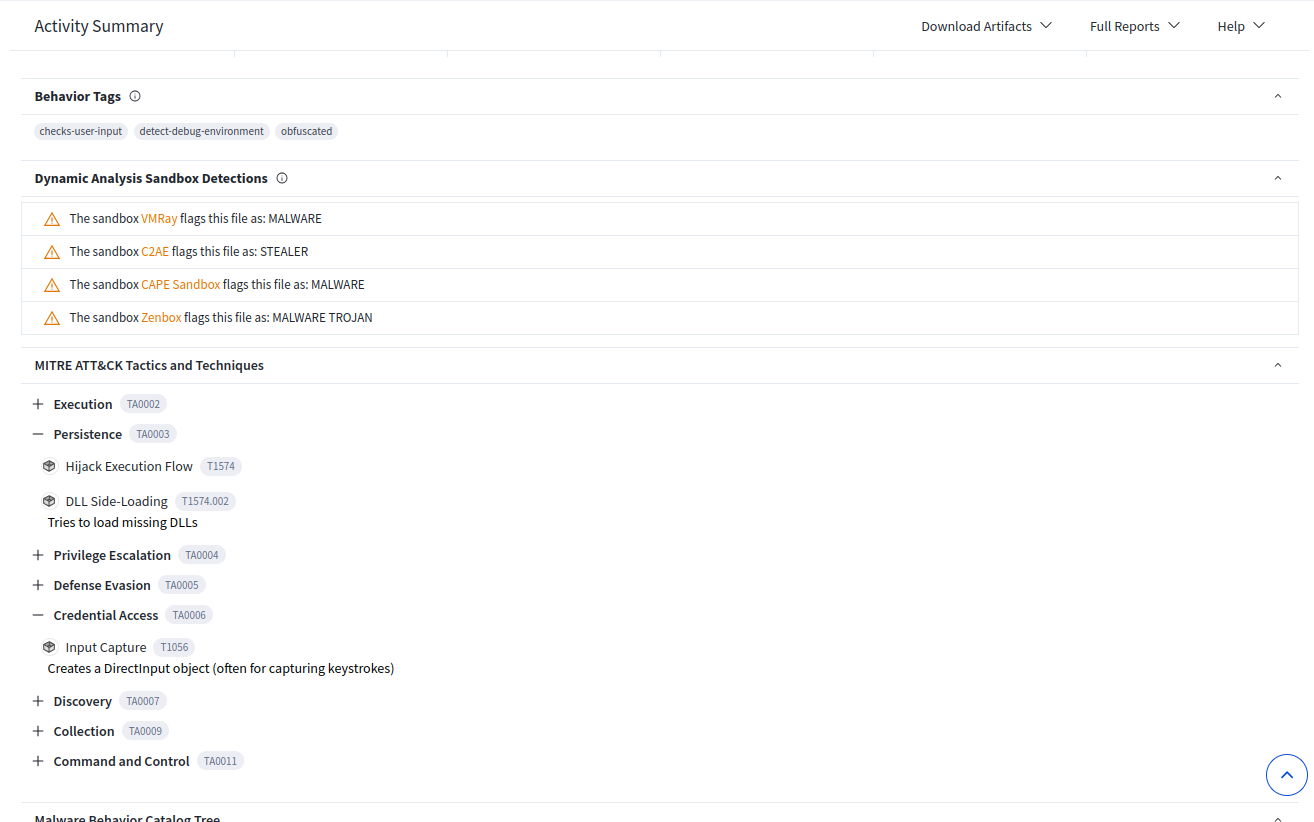
\includegraphics[scale=0.24]{images/VT_2.png}
\end{frame}


\begin{frame}[fragile]
  \frametitle{4.2 OSINT - abuse.ch - MalwareBazaar}
  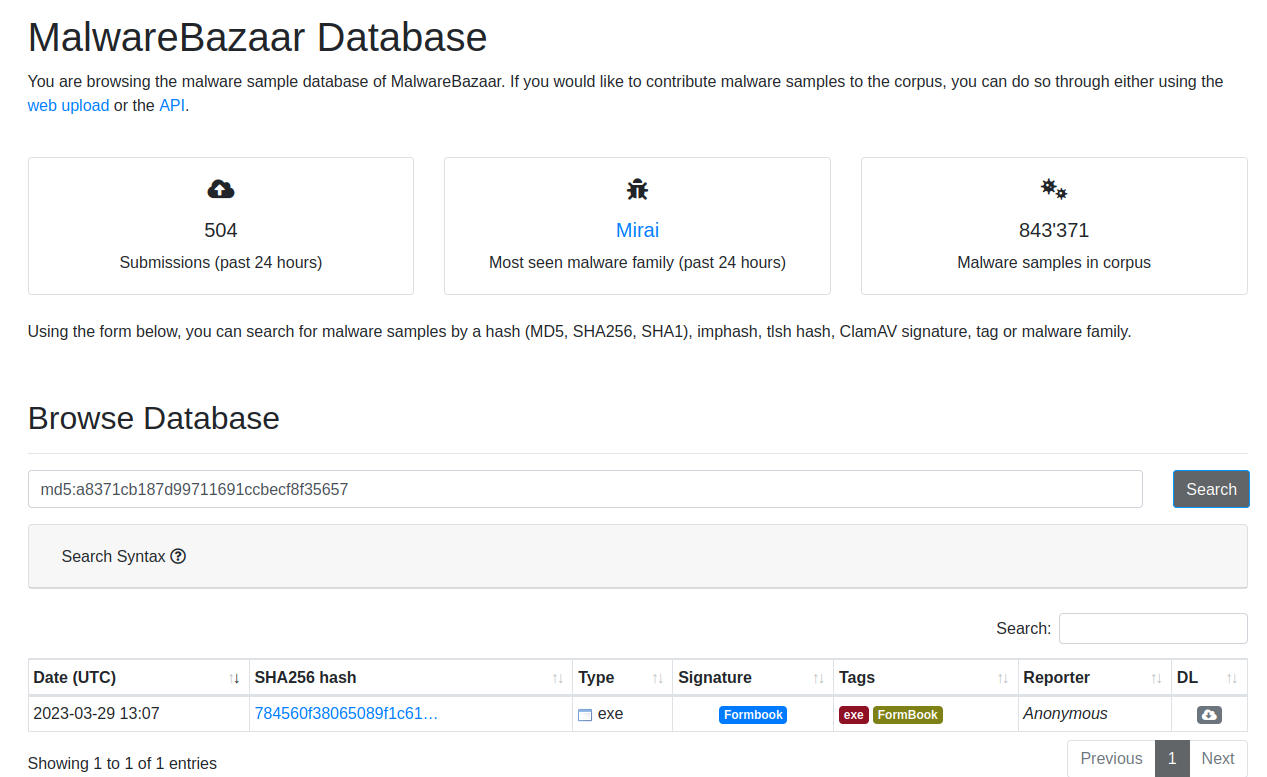
\includegraphics[scale=0.24]{images/mwBazaar.png}
\end{frame}


\begin{frame}[fragile]
  \frametitle{4.2 OSINT - MISPPriv}
  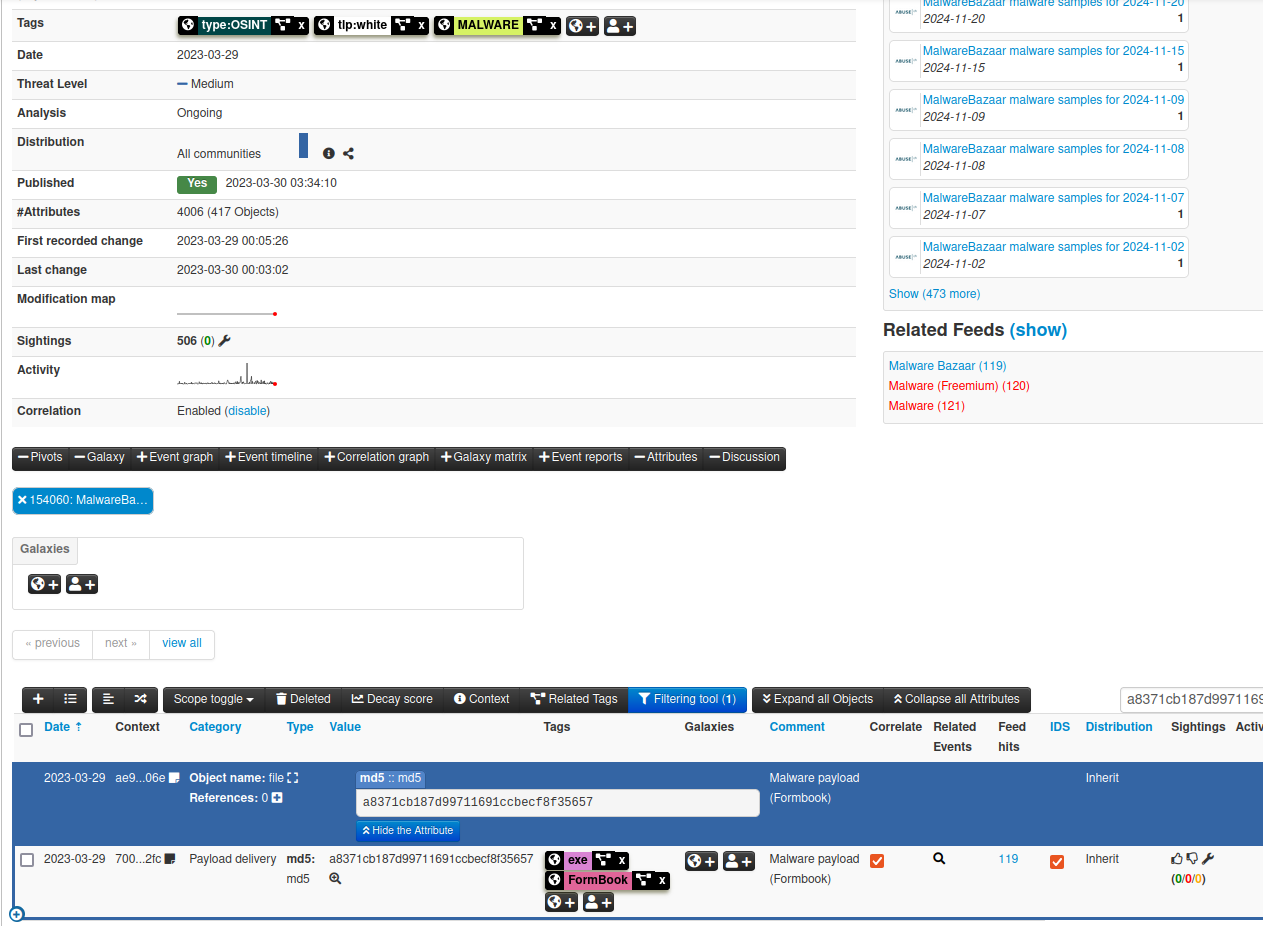
\includegraphics[scale=0.22]{images/misp.png}
\end{frame}


\begin{frame}[fragile]
  \frametitle{4.3 Sandbox - Joe}
  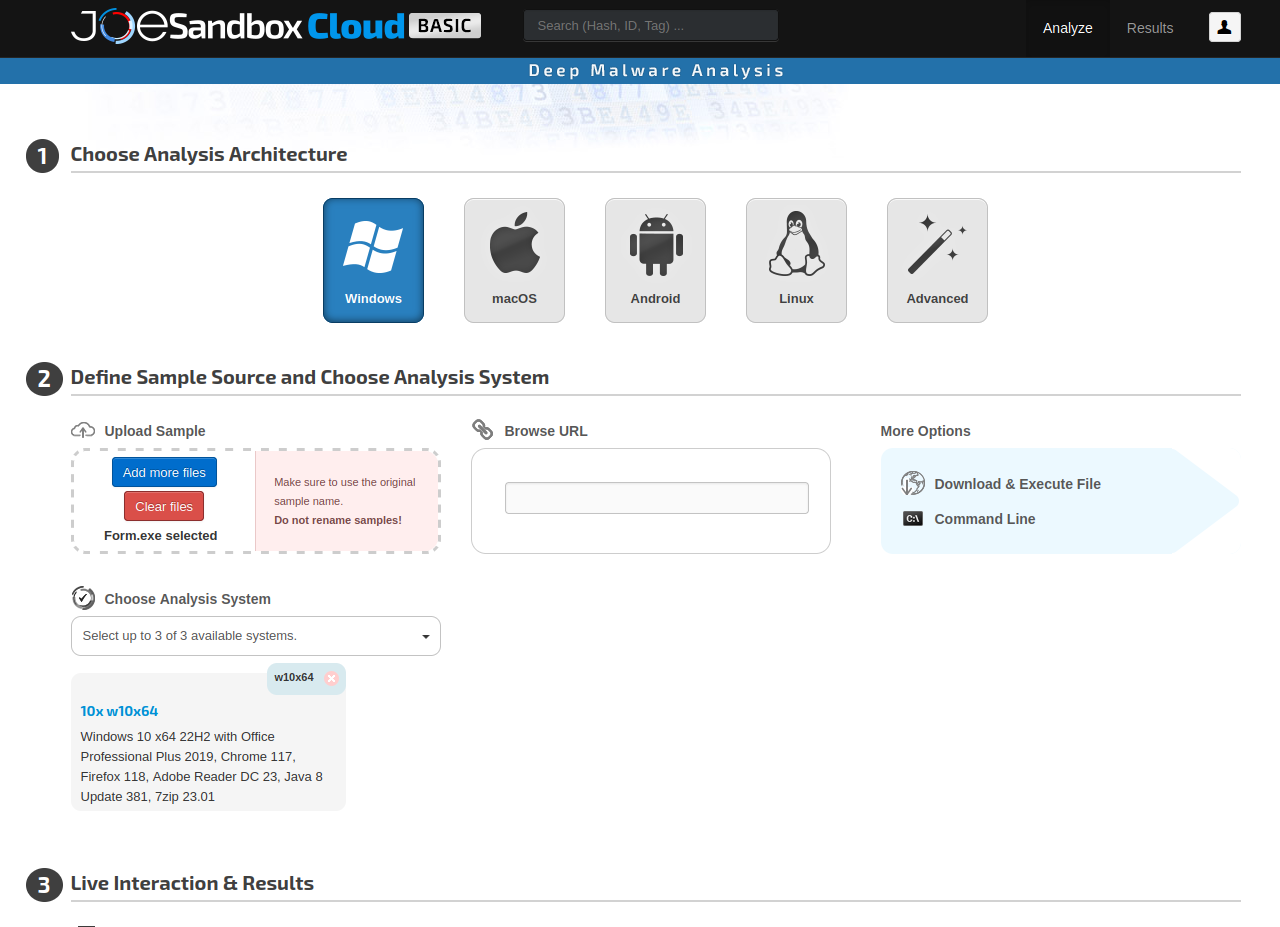
\includegraphics[scale=0.22]{images/joe1.png}
\end{frame}


\begin{frame}[fragile]
  \frametitle{4.3 Sandbox - Joe}
  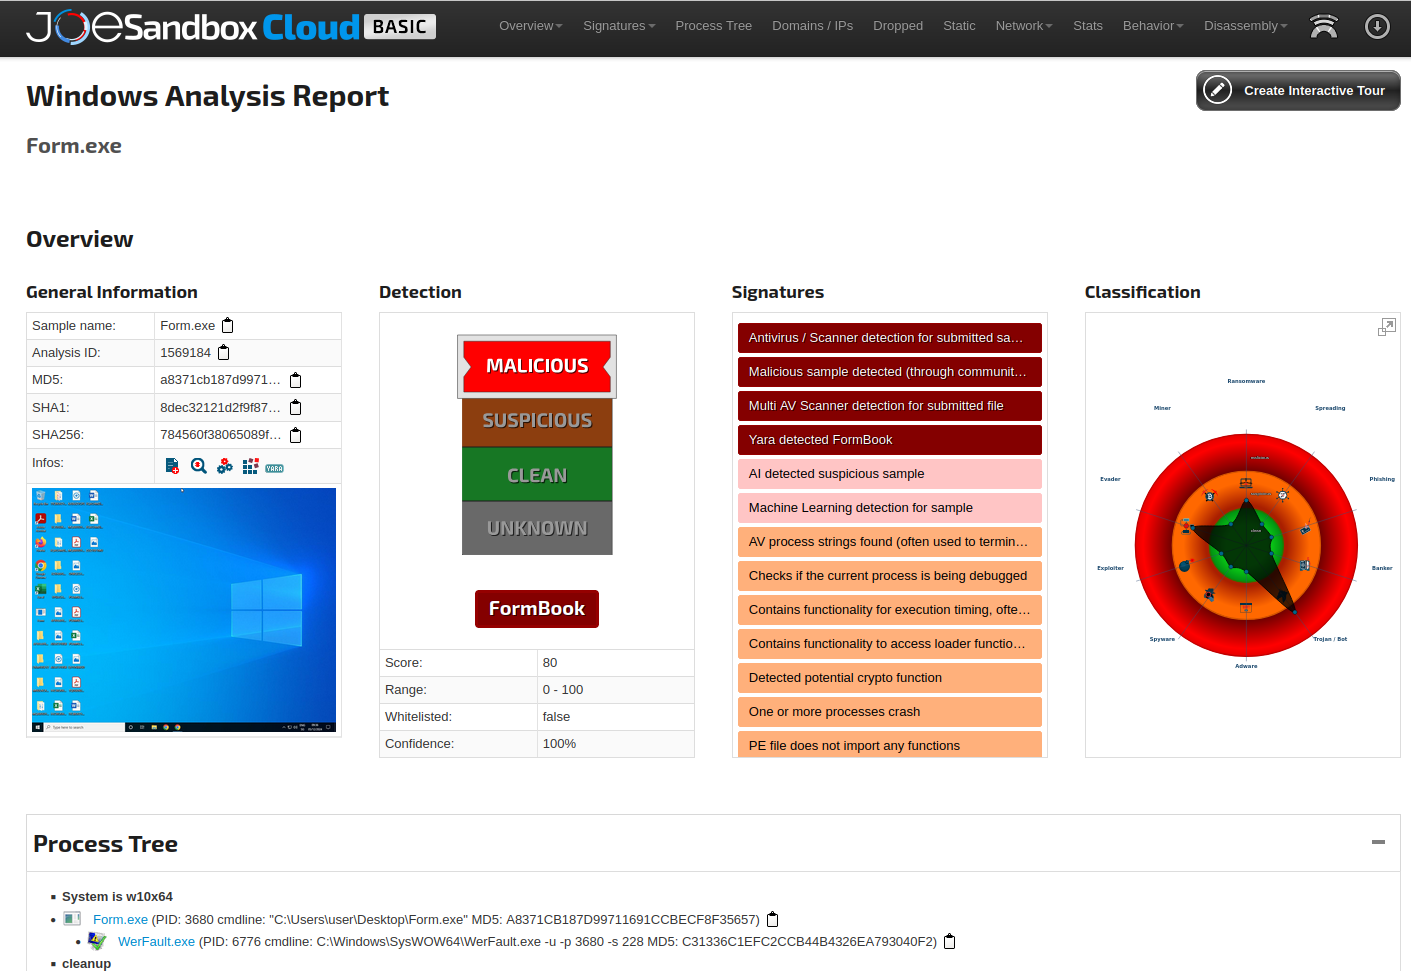
\includegraphics[scale=0.21]{images/joe2.png}
\end{frame}


\begin{frame}[fragile]
  \frametitle{4.3 Sandbox - Joe}
  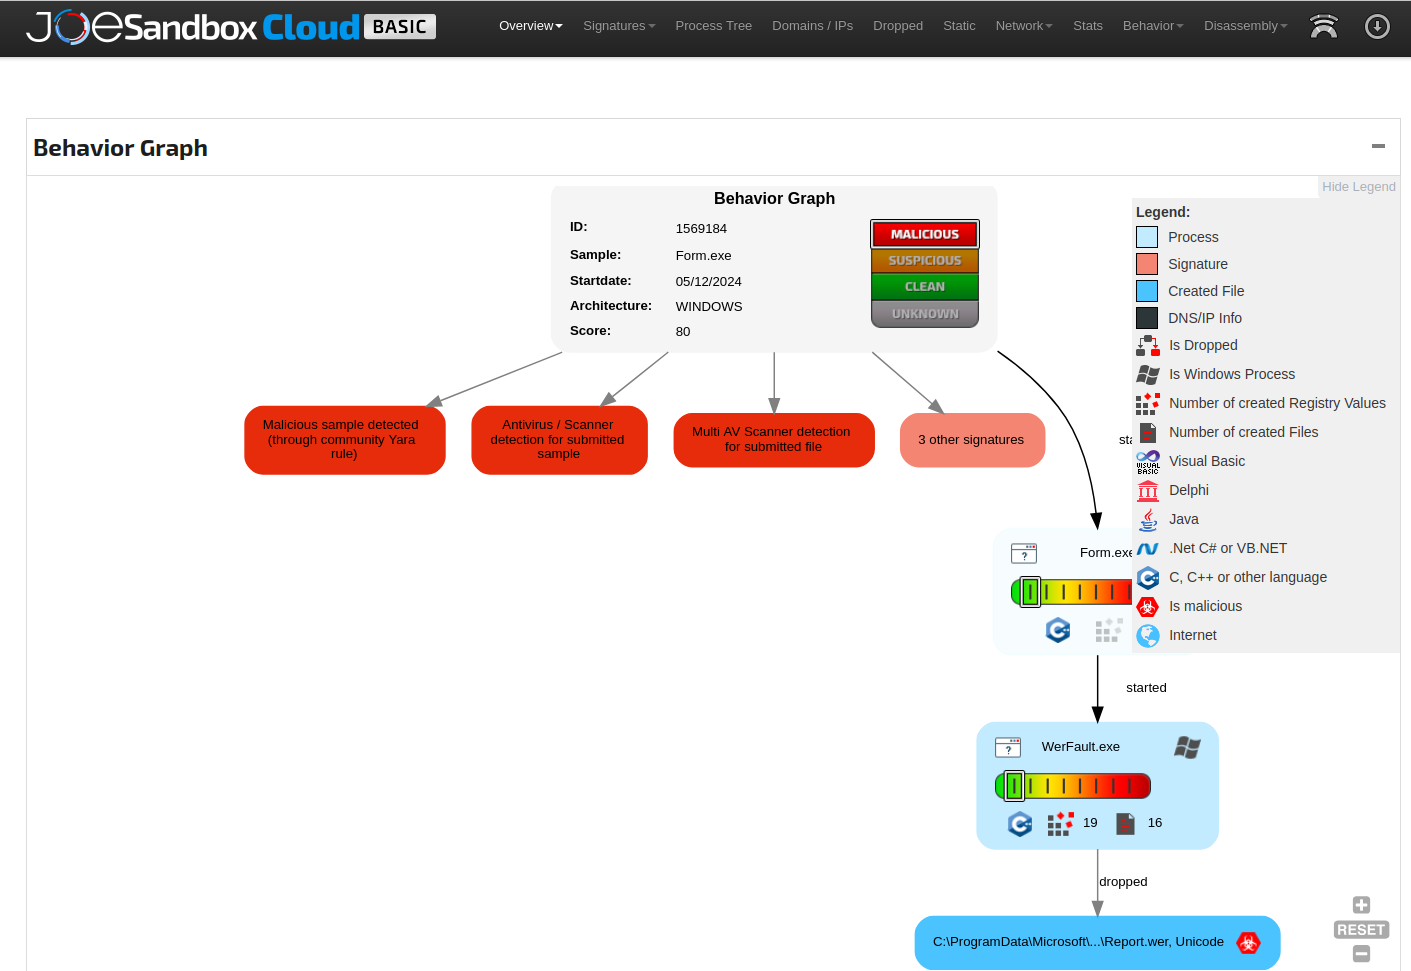
\includegraphics[scale=0.21]{images/joe3.png}
\end{frame}


\begin{frame}[fragile]
  \frametitle{4.3 Sandbox - Cuckoo3}
  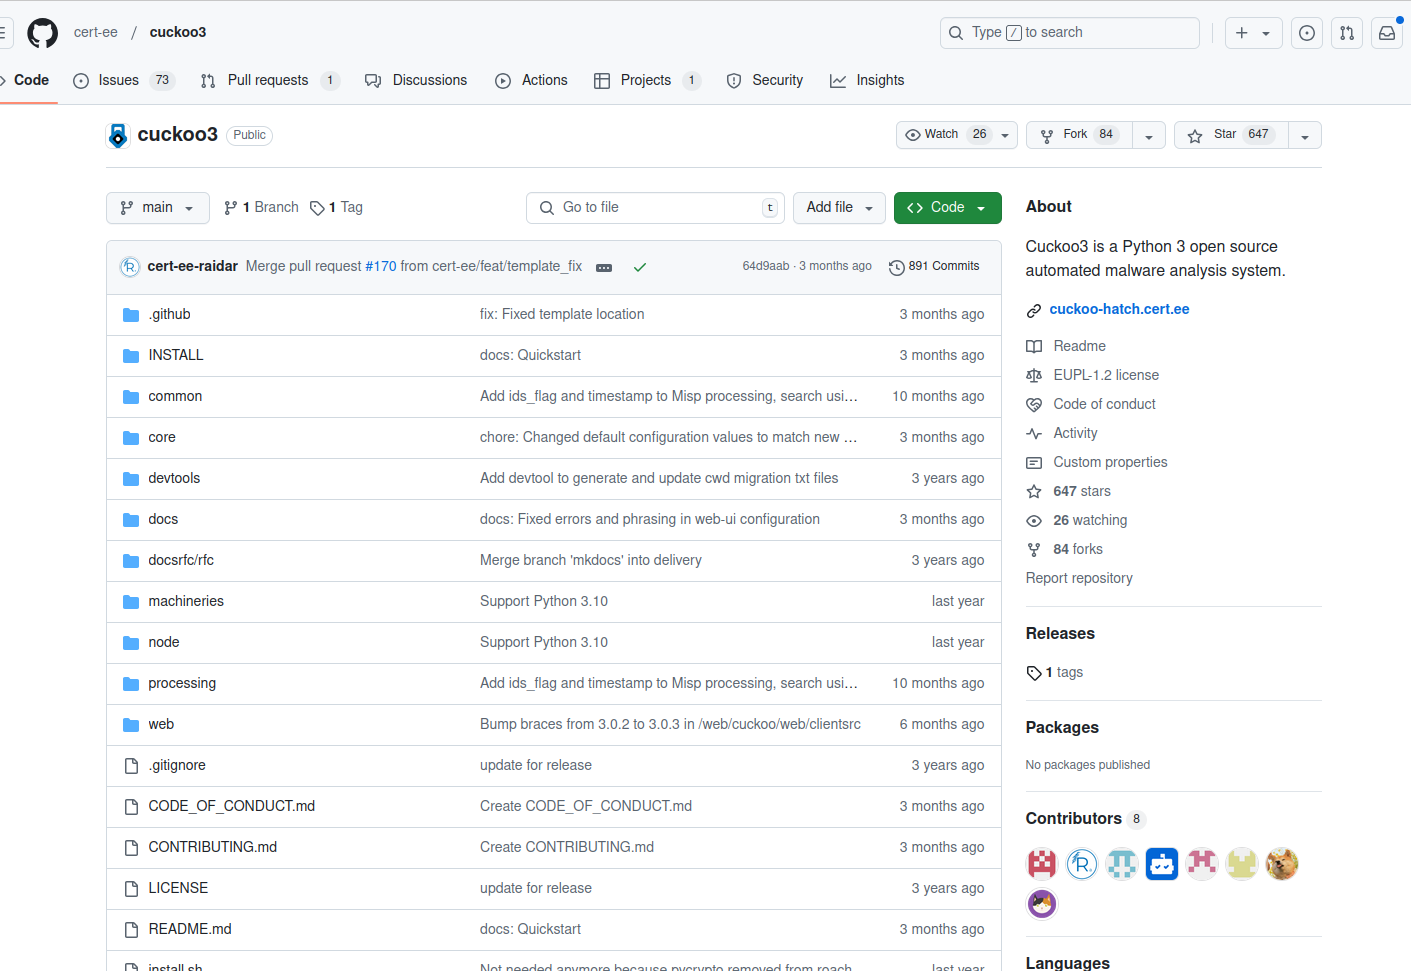
\includegraphics[scale=0.21]{images/cuckoo.png}
\end{frame}


\begin{frame}[fragile]
  \frametitle{4.4 Static Analysis}
    \begin{itemize}
        \item Malware delivery: Email
        \begin{itemize}
            \item Office documents
            \item PDF
            \item .EXE
        \end{itemize}
        \item Analyze:
        \begin{itemize}
            \item Hash values
            \item Strings
            \item Resources
            \item Imported functions
            \item Exported functions
            \item Certificate
            \item .....
        \end{itemize}
        \item[] $\to$ Capabilities of the malware
    \end{itemize}
\end{frame}


\begin{frame}[fragile]
  \frametitle{4.4 Static Analysis - Strings}
  \begin{lstlisting}[basicstyle=\tiny]
      pestr -n 7 Form.exe | less
      --------------------------
      !This program cannot be run in DOS mode.
      <Ar5<zw1<Zv
      EThis program cannot be run in DOS mode.
      :Yf/yZjP
      [)sk/Jo
      X|e^BZ8
      Rh%';,V


      pescan Form.exe
      ---------------
      file entropy:                    7.322160 (probably packed)
      fpu anti-disassembly:            no
      imagebase:                       normal
      entrypoint:                      normal
      DOS stub:                        normal
      TLS directory:                   not found
      timestamp:                       normal
      section count:                   1 (low)


      pesec Form.exe
      --------------
      ASLR:                            yes
      DEP/NX:                          yes
      SEH:                             yes
      Stack cookies (EXPERIMENTAL):    yes
  \end{lstlisting}
\end{frame}


\begin{frame}[fragile]
  \frametitle{4.4 Static Analysis - PE - Portable Execution format}
    \begin{itemize}
        \item Describe program files
        \item Contain:
        \begin{itemize}
            \item Meta data
            \item Instructions
            \item Text data
            \item Resources: Pictures and alike
        \end{itemize}
        \item Tell Windows how to load a program
        \item Provide resources to running program
        \item Provide resources like code signature
    \end{itemize}
  \begin{lstlisting}[basicstyle=\tiny]
      ---------------------------------------------
      |  1. DOS Header                            |
      |  2. PE Header                             |
      |  3. OPtional Header                       |
      |  4. Section Headers                       |
      |  5. .text Section (Program Code)          |
      |  6. .idata Section (Importd Libs)         |
      |  7. .rsrc Section (Strings, Images, ...)  |
      |  8. .reloc Section (Memory Translation)   |
      ---------------------------------------------
  \end{lstlisting}
\end{frame}


\begin{frame}[fragile]
  \frametitle{4.4 Static Analysis - PE - Basic Analysis}
  \begin{lstlisting}[basicstyle=\tiny]
file Form.exe
-------------
     Form.exe: PE32 executable (GUI) Intel 80386, for MS Windows


exiftool Form.exe
-----------------
     File Name                       : Form.exe
     File Size                       : 186 KiB
     .....
     File Type                       : Win32 EXE
     File Type Extension             : exe
     MIME Type                       : application/octet-stream
     Machine Type                    : Intel 386 or later, and compatibles
     Time Stamp                      : 2000:07:31 02:00:25+02:00
     Image File Characteristics      : Executable, 32-bit
     PE Type                         : PE32
     Linker Version                  : 11.0
     Code Size                       : 185856
     Initialized Data Size           : 0
     Uninitialized Data Size         : 0
     Entry Point                     : 0x12e0
     OS Version                      : 6.0
     Image Version                   : 0.0
     Subsystem Version               : 6.0
     Subsystem                       : Windows GUI
     Warning                         : Error processing PE data dictionary
  \end{lstlisting}
\end{frame}


\begin{frame}[fragile]
  \frametitle{4.4 Static Analysis - PE - Basic Analysis}
  \begin{lstlisting}[basicstyle=\tiny]
file Quotation.exe
------------------
     Quotation.exe: PE32 executable (GUI) Intel 80386, for MS Windows


exiftool Quotation.exe
----------------------  
     ...
     Machine Type                    : Intel 386 or later, and compatibles
     Time Stamp                      : 2005:08:14 14:47:46+02:00
     PE Type                         : PE32
     Linker Version                  : 6.0
     Code Size                       : 647168
     Initialized Data Size           : 32768
     Uninitialized Data Size         : 0
     Entry Point                     : 0x15f4
     OS Version                      : 4.0
     Character Set                   : Unicode
     Comments                        : Natcher
     Company Name                    : Glucosazone
     Legal Copyright                 : CRUSTER3
     Legal Trademarks                : Forearming
     Product Name                    : UNKLE
     File Version                    : 1.02.0009
     Product Version                 : 1.02.0009
     Internal Name                   : Aurous
     Original File Name              : Aurous.exe
  \end{lstlisting}
\end{frame}


\begin{frame}[fragile]
  \frametitle{4.4 Static Analysis - PE - Header}
  \begin{lstlisting}[basicstyle=\tiny]
readpe -H Form.exe
------------------

     DOS Header
         Magic number:                    0x5a4d (MZ)
         Bytes in last page:              144
         Pages in file:                   3
         .....

     Optional/Image header
         Magic number:                    0x10b (PE32)
         Linker major version:            11
         Linker minor version:            0
         Size of .text section:           0x2d600
         Size of .data section:           0
         Size of .bss section:            0
         Entrypoint:                      0x12e0
         Address of .text section:        0x1000
         Address of .data section:        0x2f000
         ImageBase:                       0x400000
         Alignment of sections:           0x1000
         Alignment factor:                0x200
         .....
	 Size of image:                   0x2f000
         Size of headers:                 0x200
         Checksum:                        0
         Subsystem required:              0x2 (IMAGE_SUBSYSTEM_WINDOWS_GUI)
         DLL characteristics:             0x8140
         .....
  \end{lstlisting}
\end{frame}


\begin{frame}[fragile]
  \frametitle{4.4 Static Analysis - PE - Imported Functions}
  \begin{lstlisting}[basicstyle=\tiny]
readpe -i ../1.exe
------------------
    Library
        Name:                            COMCTL32.dll
        Functions
                Name:                            ImageList_GetDragImage
                Name:                            ImageList_Merge
                Name:                            ImageList_SetOverlayImage
                Name:                            UninitializeFlatSB
                Name:                            ImageList_DragEnter
    Library
        Name:                            OLEAUT32.dll
        Functions
            Function
                Ordinal:                         294
    Library
        Name:                            ADVAPI32.dll
        Functions
                Name:                            RegOpenKeyExA
                Name:                            MapGenericMask
                Name:                            AdjustTokenGroups
                Name:                            SetSecurityDescriptorDacl
                Name:                            GetSecurityDescriptorLength
                Name:                            StartServiceA
                Name:                            OpenServiceA
    Library
        Name:                            MSVCRT.dll
        Functions
                Name:                            _mbsspnp
         .....
  \end{lstlisting}
\end{frame}


\begin{frame}[fragile]
  \frametitle{4.4 Static Analysis - PE - Resources}
  \begin{lstlisting}[basicstyle=\tiny]
wrestool -l ../1.exe
--------------------

--type=3 --name=23166 --language=2064 [type=icon offset=0x398cd8 size=455]
--type=3 --name=23167 --language=2064 [type=icon offset=0x398e78 size=648]
--type=3 --name=23168 --language=2064 [type=icon offset=0x398f78 size=642]
--type=3 --name=23169 --language=2064 [type=icon offset=0x399118 size=671]
--type=3 --name=23170 --language=2064 [type=icon offset=0x399358 size=1152]
--type=3 --name=23171 --language=2064 [type=icon offset=0x3995d8 size=1401]
--type=3 --name=23172 --language=2064 [type=icon offset=0x399a18 size=739]
--type=5 --name=34145 --language=2064 [type=dialog offset=0x398740 size=426]
--type=5 --name=34146 --language=2064 [type=dialog offset=0x3988f0 size=382]
--type=5 --name=34147 --language=2064 [type=dialog offset=0x398a70 size=562]
--type=9 --name=44061 --language=2064 [type=accelerator offset=0x3986e8 size=88]
--type=0 --name=5676 --language=2064 [offset=0x398ca8 size=11]
--type=0 --name=5677 --language=2064 [offset=0x398cb8 size=30]
--type=0 --name=5678 --language=2064 [offset=0x399c58 size=219344]
--type=0 --name=5679 --language=2064 [offset=0x3cf528 size=3852]
--type=14 --name=63607 --language=2064 [type=group_icon offset=0x398e60 size=20]
--type=14 --name=63608 --language=2064 [type=group_icon offset=0x398f60 size=20]
--type=14 --name=63609 --language=2064 [type=group_icon offset=0x399100 size=20]
--type=14 --name=63610 --language=2064 [type=group_icon offset=0x399340 size=20]
--type=14 --name=63611 --language=2064 [type=group_icon offset=0x3995c0 size=20]
--type=14 --name=63612 --language=2064 [type=group_icon offset=0x399a00 size=20]
--type=14 --name=63613 --language=2064 [type=group_icon offset=0x399c40 size=20] 
  \end{lstlisting}
\end{frame}


\begin{frame}[fragile]
  \frametitle{4.4 Static Analysis - Considerations}
    \begin{itemize}
        \item Perfect disassembly $\to$ Unsolved problem
        \item Linear disassembly
        \begin{itemize}
            \item Identify the program code
            \item Decode the bytes
        \end{itemize}
        \item Linear disassembly limitations
        \begin{itemize}
            \item Don't know how instructions get decoded by CPU
            \item Could not counter fight obfuscation
        \end{itemize}
        \item Obfuscation techniques
        \begin{itemize}
            \item Packing
            \item Resource Obfuscation
            \item Anti-Disassembly
            \item Dynamic Data Download
        \end{itemize}
        \item Counter fight obfuscation
        \begin{itemize}
            \item Dynamic Analysis
            \item Run malware in isolated environment
        \end{itemize}
    \end{itemize}
\end{frame}


\begin{frame}[fragile]
  \frametitle{4.5 x86 Assembly: General-Purpose Registers}
    \begin{figure}
        \includegraphics[scale=0.34]{images/x86-registers.png}
        \captionsetup{labelformat=empty,labelsep=none}
        \transparent{0.7}%
        \caption[]{\tiny https://www.cs.virginia.edu/~evans/cs216/guides/x86.html}
    \end{figure}
\end{frame}


\begin{frame}[fragile]
  \frametitle{4.5 x86 Assembly: Stack and Control Flow Registers}
    \begin{figure}
        \includegraphics[scale=0.34]{images/x86-registers.png}
        \captionsetup{labelformat=empty,labelsep=none}
        \transparent{0.7}%
        \caption[]{\tiny https://www.cs.virginia.edu/~evans/cs216/guides/x86.html}
    \end{figure}
\end{frame}


\begin{frame}[fragile]
  \frametitle{4.5 x86 Assembly: Instructions}
  \begin{lstlisting}[basicstyle=\tiny]
Arithmetic:      add ebx, 100       Adds 100 to the value in EBX
                 sub ecx, 123       Substract 123 from the value in ECX
	         inc ah             Increments value in AH by 1
	         dec al             Decrements value in AL by 1

Data Movement:   mov eax, ebx       Move value in EBX into register EAX
                 mov eax, [0x4711]  Move value at memory 0x4711 intp EAX
		 mov eax, 1         Move the value 1 into register EAX
		 mov [0x4711], eax  Move value of EAX into memory 0x4711

Stack:           push 1             Increment ESP; Store 1 on top of stack
                 pop eax            Store highest value in EAX; Decrement ESP

Control Flow:    call [address]     1. Put EIP on top of the stack
                                    2. Put [address] into EIP
                 ret                1. Popped top of teh stack into EIP
		                    2. Resume execution
		 jmp 0x1234         Start executing progamm code at 0x1234
		 cmp eax, 100       1. Compares value in EAX with 100
		                    2. Based on result set EFLAGS register
		 jge 0x1234         1. Interpret EFLAGS register
		                    2. If 'greater' or 'equal' flag then jump
  \end{lstlisting}
\end{frame}


\begin{frame}[fragile]
  \frametitle{4.5 x86 Assembly: Control Flow Graphs}
  \begin{lstlisting}[basicstyle=\tiny]
start:             Symbol for address of next instruction
mov eax, 3         Initialize a counter of 3 into EAX

loop:              Symbol for address of next instruction
sub eax, 1         Substract 1 from value in EAX
cmp 0, eax         Compare value in EAX with 0; Set EFLAGS
jne $loop          IF EFLAGS 'not equal' jump to 'loop'

end:               Symbol for address of next instruction
mov eax, 12











.
  \end{lstlisting}
\end{frame}


\begin{frame}[fragile]
  \frametitle{4.5 x86 Assembly: Control Flow Graphs}
  \begin{lstlisting}[basicstyle=\tiny]
start:             Symbol for address of next instruction
mov eax, 3         Initialize a counter of 3 into EAX

loop:              Symbol for address of next instruction
sub eax, 1         Substract 1 from value in EAX
cmp 0, eax         Compare value in EAX with 0; Set EFLAGS
jne $loop          IF EFLAGS 'not equal' jump to 'loop'

end:               Symbol for address of next instruction
mov eax, 12


      -------------    ------>    -------------    ------>    ------------- 
     | start:      |      --->   | loop:       |             | end:        |
     | ----------- |     |       | ----------- |             | ----------- |
     |             |     |       |             |             |             |
     | mov eax, 3  |     |       | sub eax, 1  |             | mov eax, 12 |
     |             |     |       | cmp 0, eax  |             |             |
      -------------       ----   | jne $loop   |              -------------
			         |             | 
			          ------------- 
.
  \end{lstlisting}
\end{frame}







